\chapter{Analiza jakości dopasowania śladów w oparciu o test $\chi^2$}
\section{Selekcja przypadków}
W celu wykonania analizy jakości dopasowania śladów posłużono się rozpadem 
\begin{equation}
B_d \rightarrow J/\Psi(\rightarrow \mu +\mu) + K_s(\rightarrow \pi + \pi )
\end{equation}

Jest to rozpad pół leptonowy, który da się opisać przy użyciu diagramu Feynmana zamieszczonego na rysunku \ref{rys:BJPsi}.

 \begin{figure}[h]
 \centering
 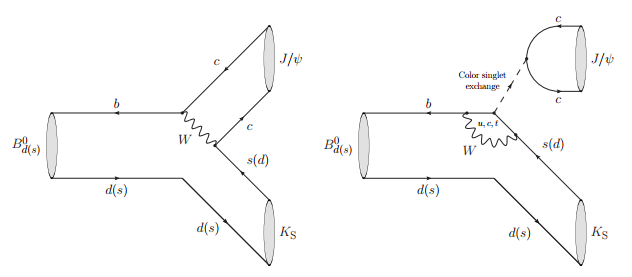
\includegraphics[scale=0.8]{rozdzial6/Feynman.png}
 % GAUDI.jpeg: 767x379 pixel, 96dpi, 20.29x10.03 cm, bb=0 0 575 284
 \caption{Diagramy Feynmana obrazujące topologię rozpadu $B_d \rightarrow J/\Psi(\rightarrow \mu +\mu) + K_s(\rightarrow \pi + \pi )$. po lewej diagram typu drzewiastego, po prawej typu pingwin. }
 \label{rys:BJPsi}
\end{figure}

Faktem, wartym podkreślenia jest, że w podczas analizy wzięto pod uwagę przypadki w których z produktami rozpadów mezonu $K_s$, czyli pionami, stowarzyszono ślady zarówno długie jak i typu "Downstream".
\section{Analiza bazująca an symulacjach Monte Carlo} 
Ten podrozdział zawiera wyniku uzyskane dla symulowanych danych Monte Carlo. Analiza oparta na tego typu danych jest istotna, gdyż ewentualna niezgodność wyników może wskazywać na problemy w pracy detektora. 
\subsection{Wydajność rekonstrukcji śladów}
Pierwszym elementem pracy w analizie jakości dopasowania śladów w eksperymencie LHCb jest zbadanie wydajności rekonstrukcji śladów. Jest to bardzo istotna analiza, która w bardzo szybko sposób obrazuje jaki ułamek rekonstruowanych śladów jest związany z interesującym rozpadem. Z praktycznego punktu widzenia wydajność (ang. efficiency) jest wyliczana przy wykorzystaniu informacji dotyczącej numeru pdg cząstki \cite{PDG}. natomiast formalna, matematyczna definicja jest realizowana przy użyciu zależności:

\begin{eqnarray}
\varepsilon &=& \frac{\# sladów\_jezeli\_nr\_pdg\_rodzica\_jest\_odpowiedni }{\# wszystkich\_sladów} \\ \nonumber &=&\frac{a_{total}}{n_{total}}
\end{eqnarray}
Natomiast niepewność wyznaczenia tej wielkości przyjmuje się jako:
\begin{equation}
\sigma_{\varepsilon}=\frac{\sqrt{a_{total}(1-\varepsilon)}}{n_{total}}
\end{equation}

\begin{figure}[H]
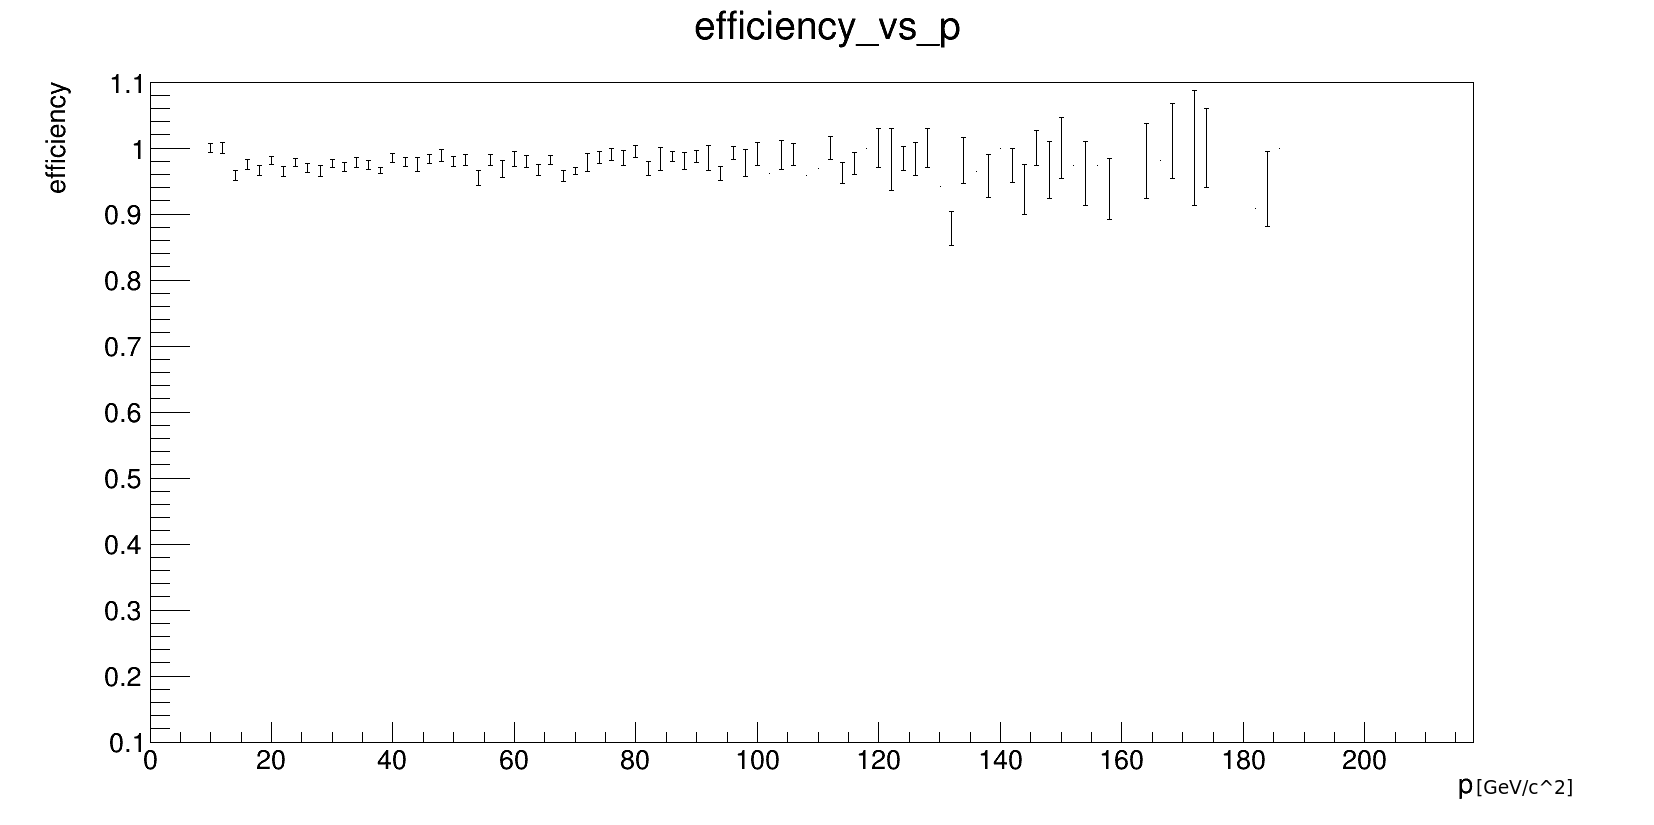
\includegraphics[scale=0.25]{rozdzial6/Jpsi_p.png} \\
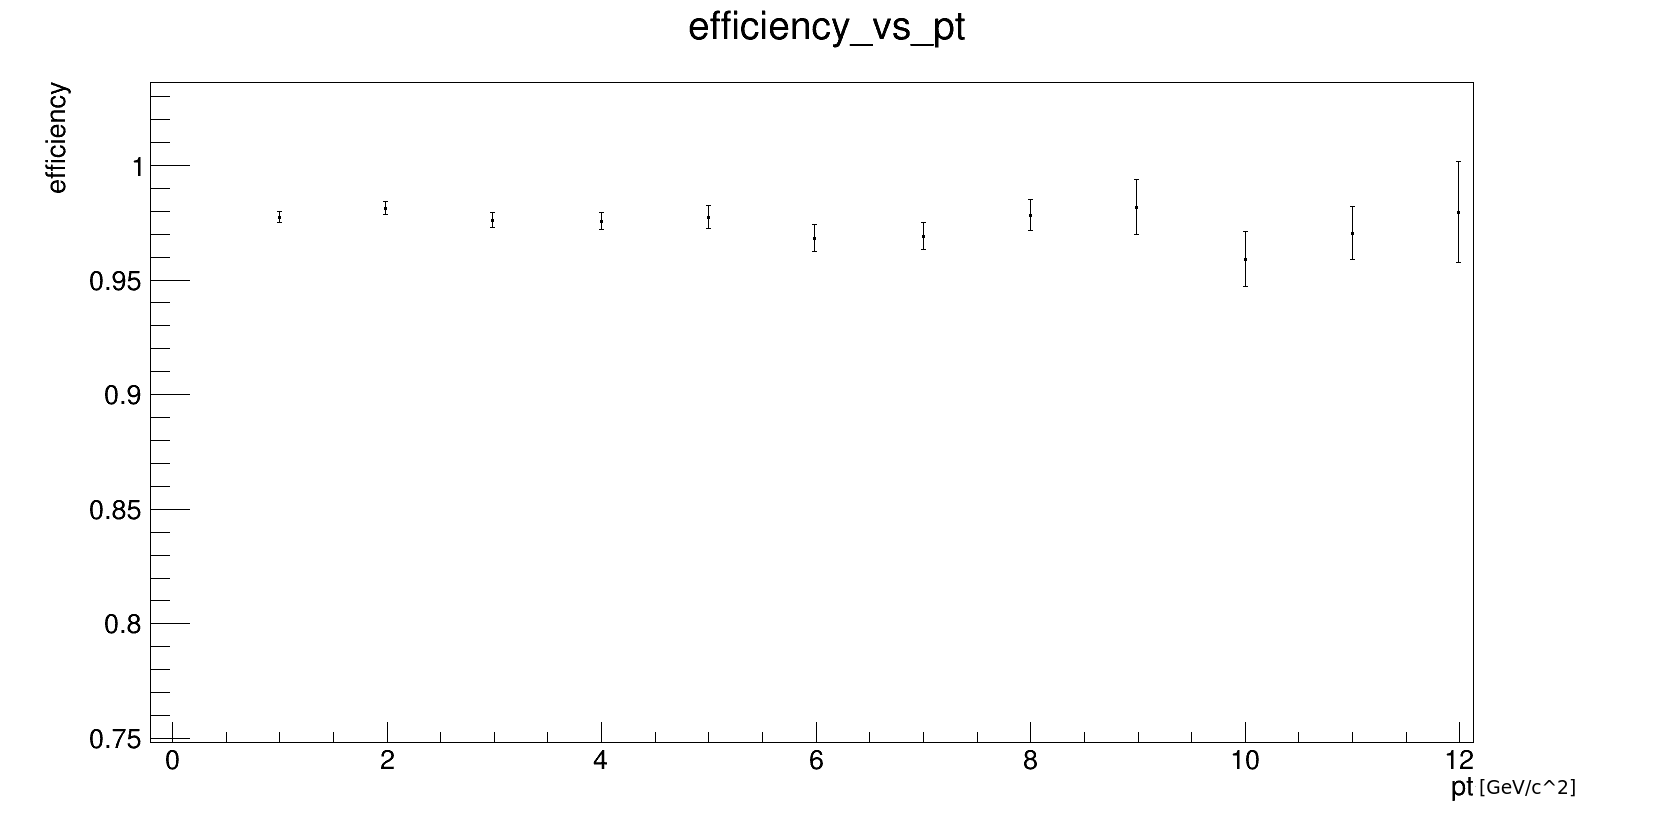
\includegraphics[scale=0.25]{rozdzial6/Jpsi_pt.png} \\
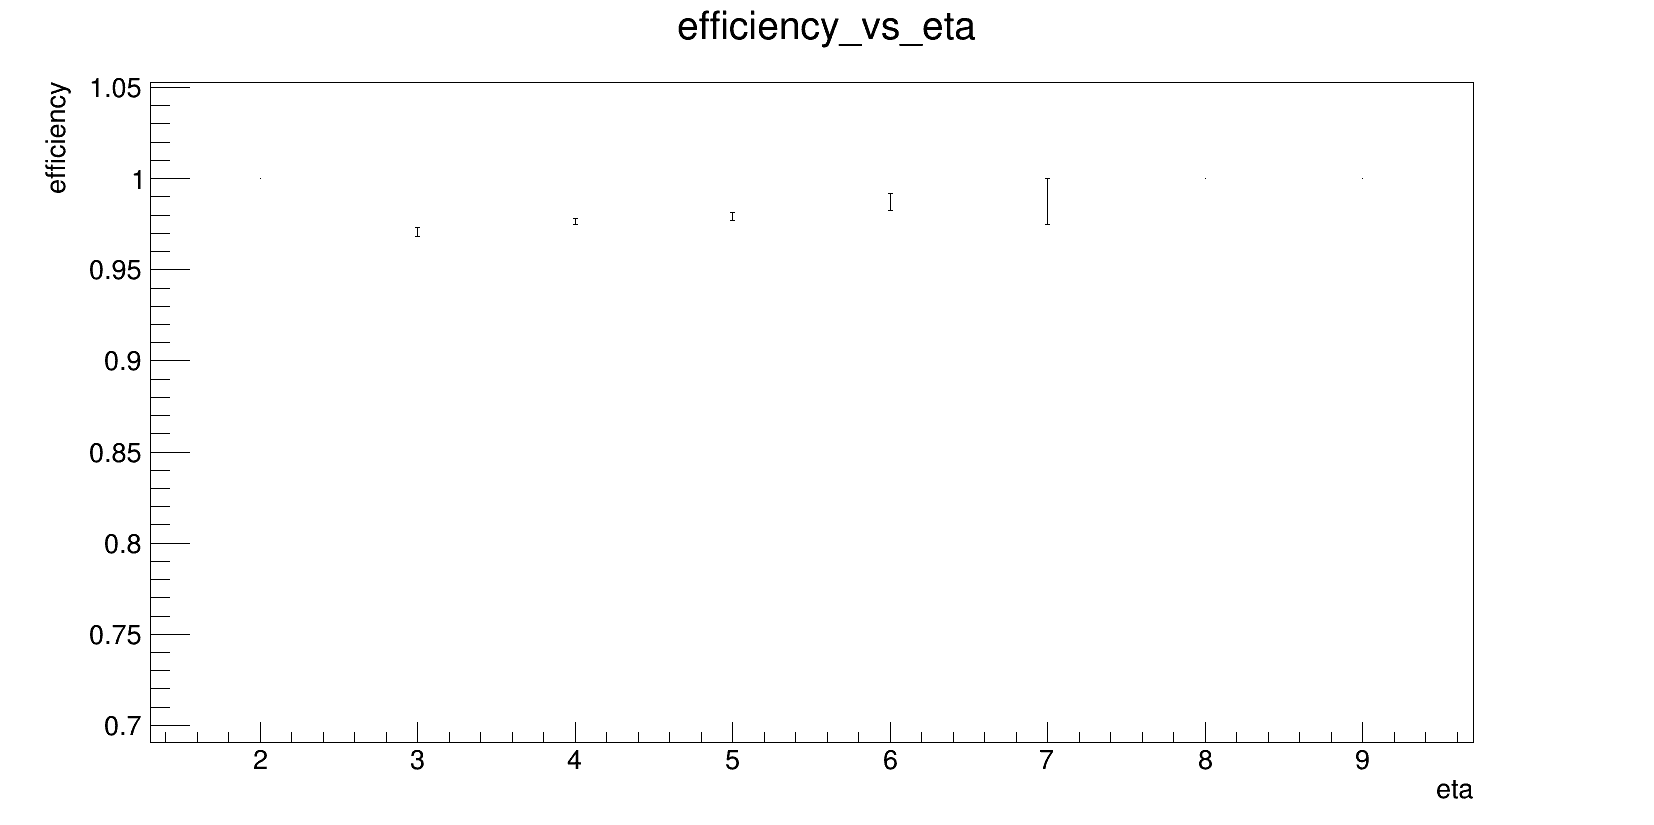
\includegraphics[scale=0.25]{rozdzial6/Jpsi_eta.png} \\ 
\caption{Wydajność rekonstrukcji śladów długich zrekonstruowanych dla cząstek z rozpadu $J/\Psi \rightarrow \mu + \mu $  w funkcji pędu (góra), pędu poprzecznego (środek) oraz pseudorapidity (dół).}
\label{effJPsi}
\end{figure}



\begin{figure}[H]
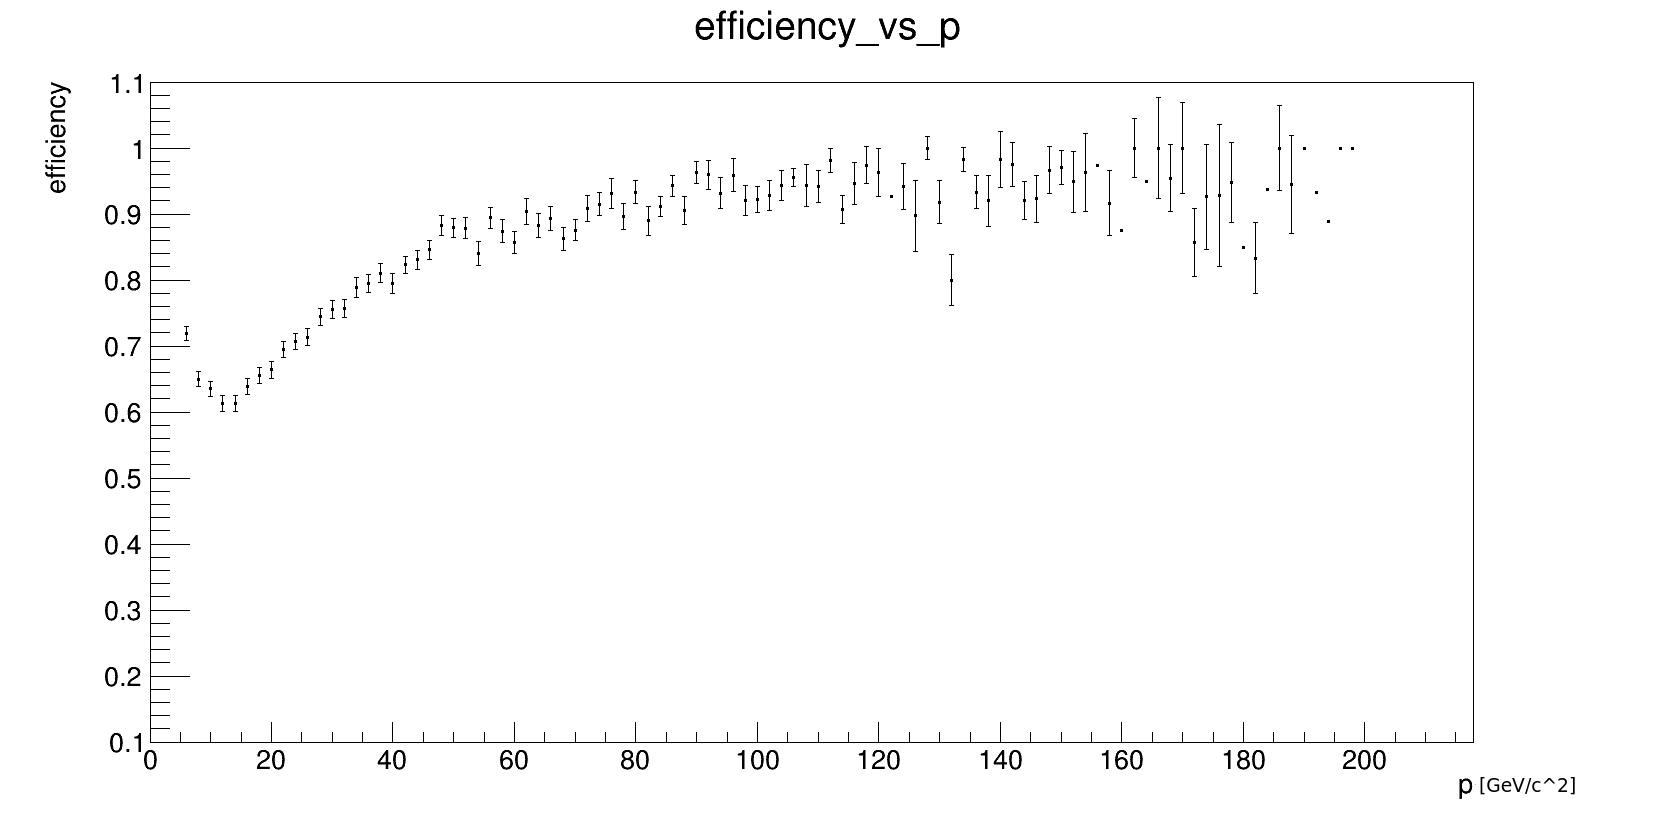
\includegraphics[scale=0.25]{rozdzial6/KsLL_p.png} \\
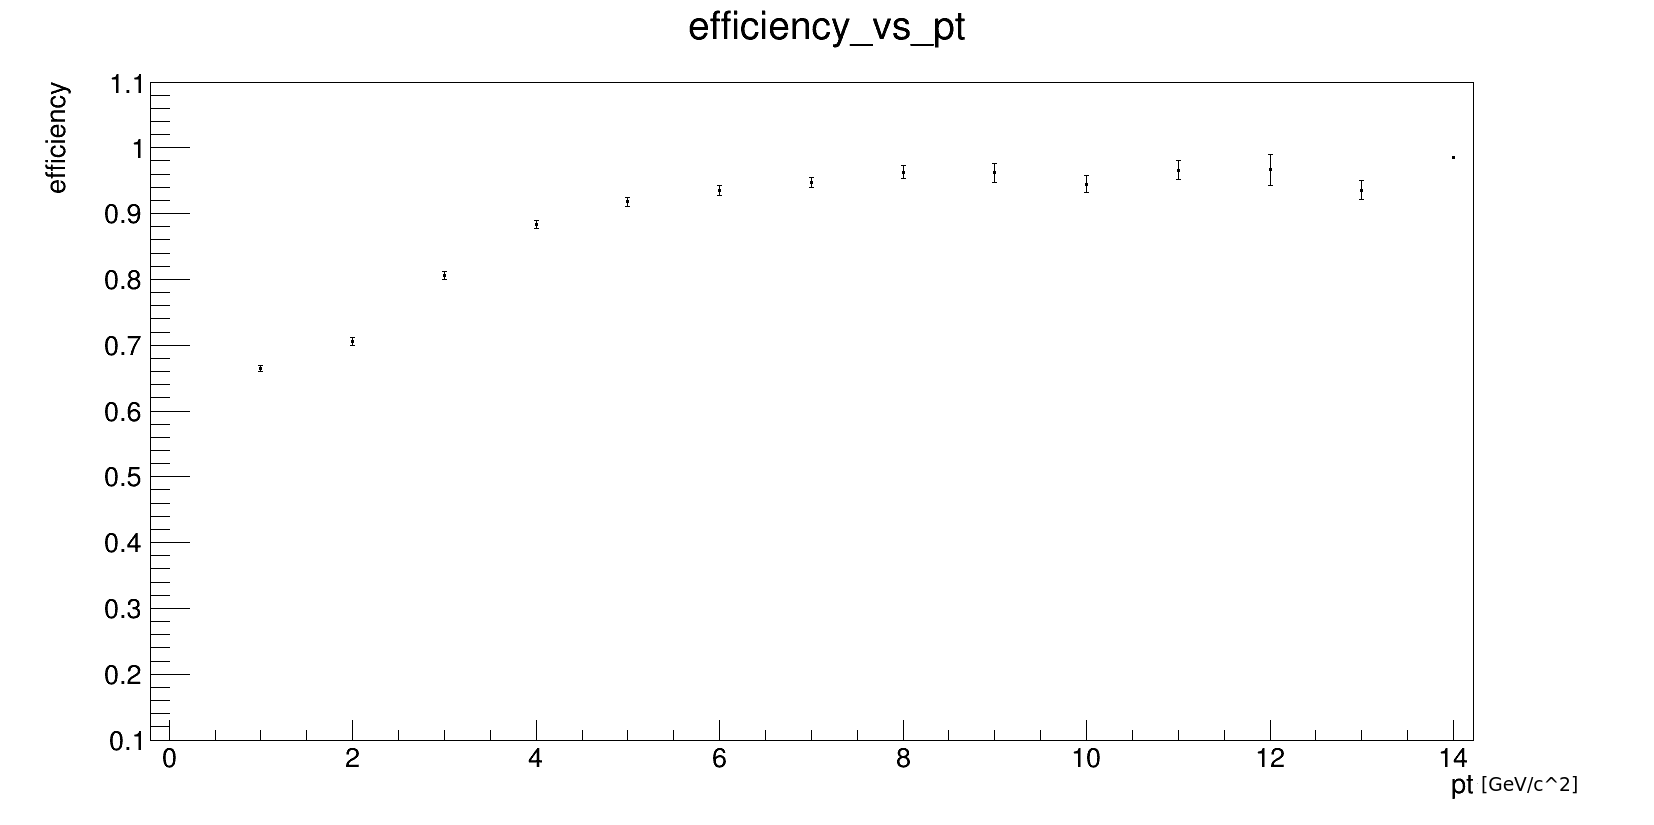
\includegraphics[scale=0.25]{rozdzial6/KsLL_pt.png} \\
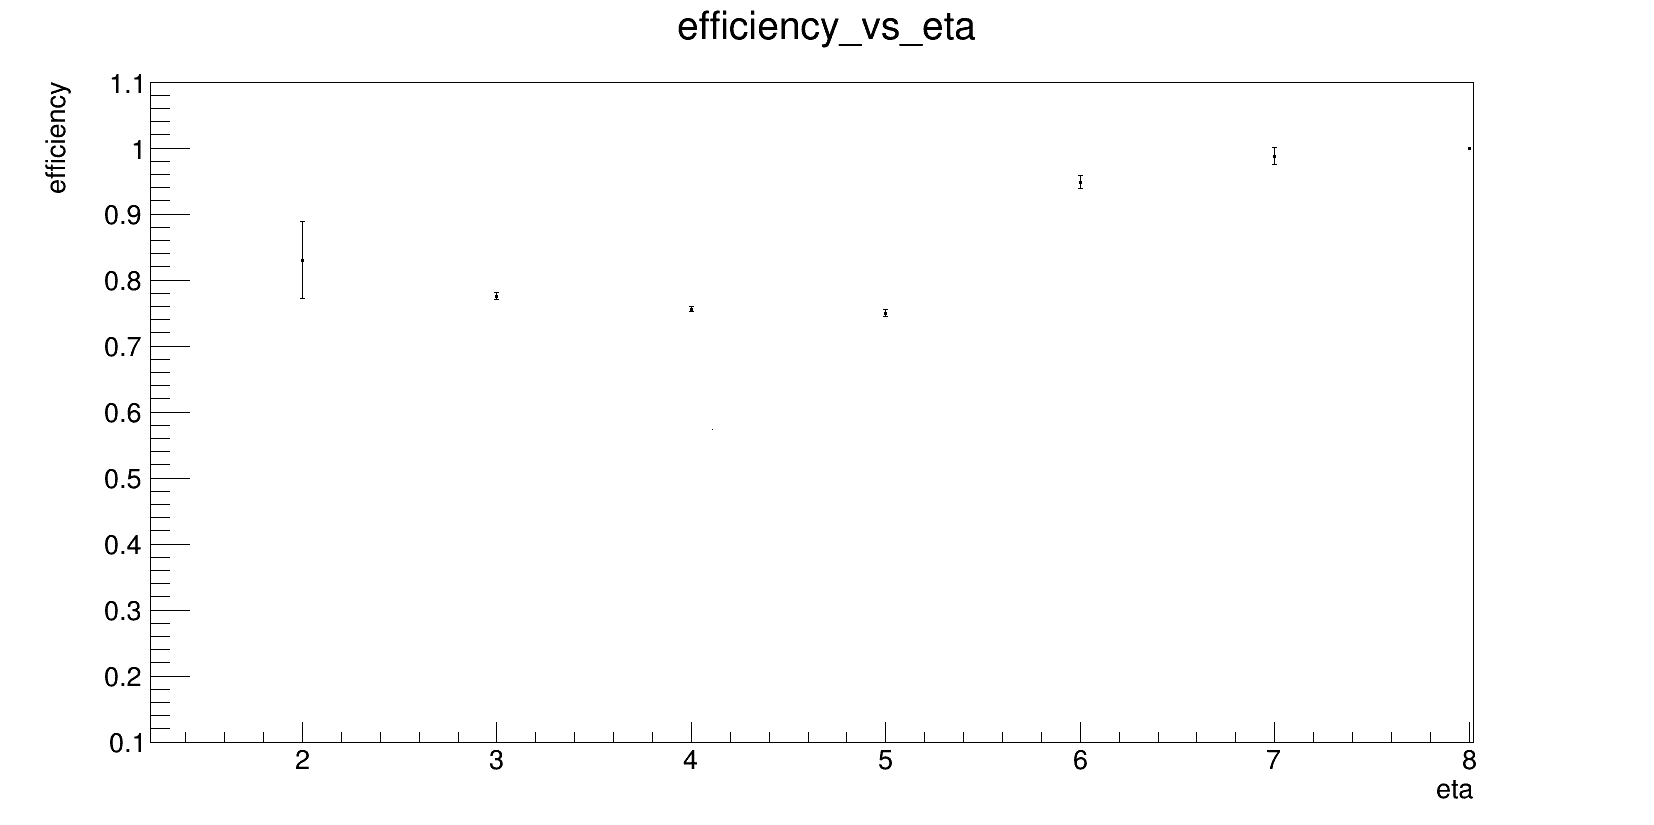
\includegraphics[scale=0.25]{rozdzial6/KsLL_eta.png} \\ 
\caption{Wydajność rekonstrukcji śladów długich zrekonstruowanych dla cząstek z rozpadu $K_s \rightarrow \pi + \pi $  w funkcji pędu (góra), pędu poprzecznego (środek) oraz pseudorapidity (dół).}
\label{KsLL}
\end{figure}

\begin{figure}[H]
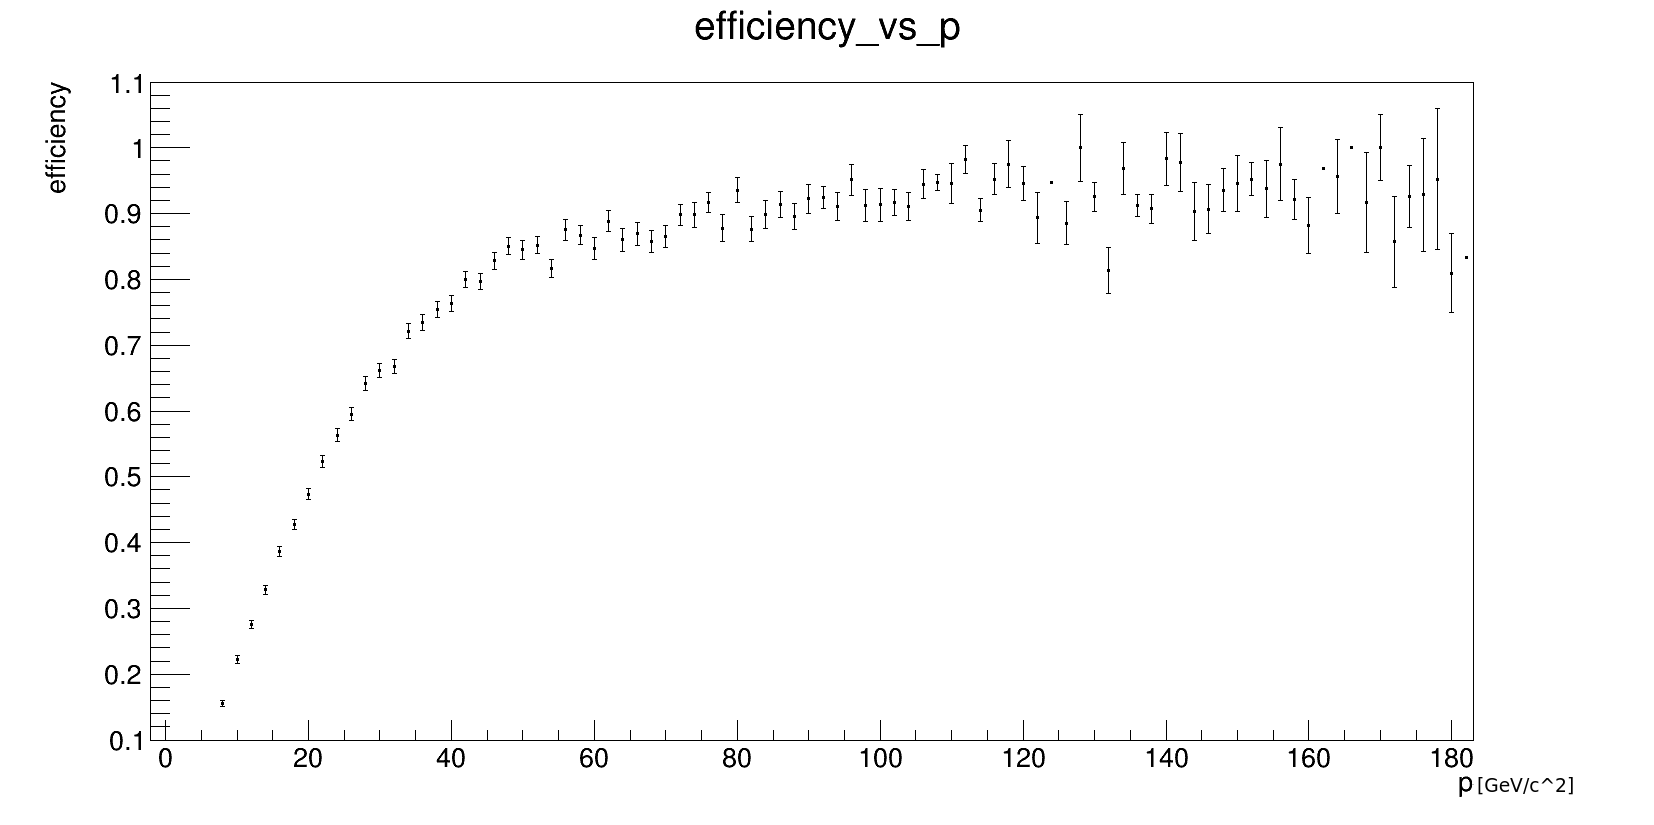
\includegraphics[scale=0.25]{rozdzial6/KsDD_p.png} \\
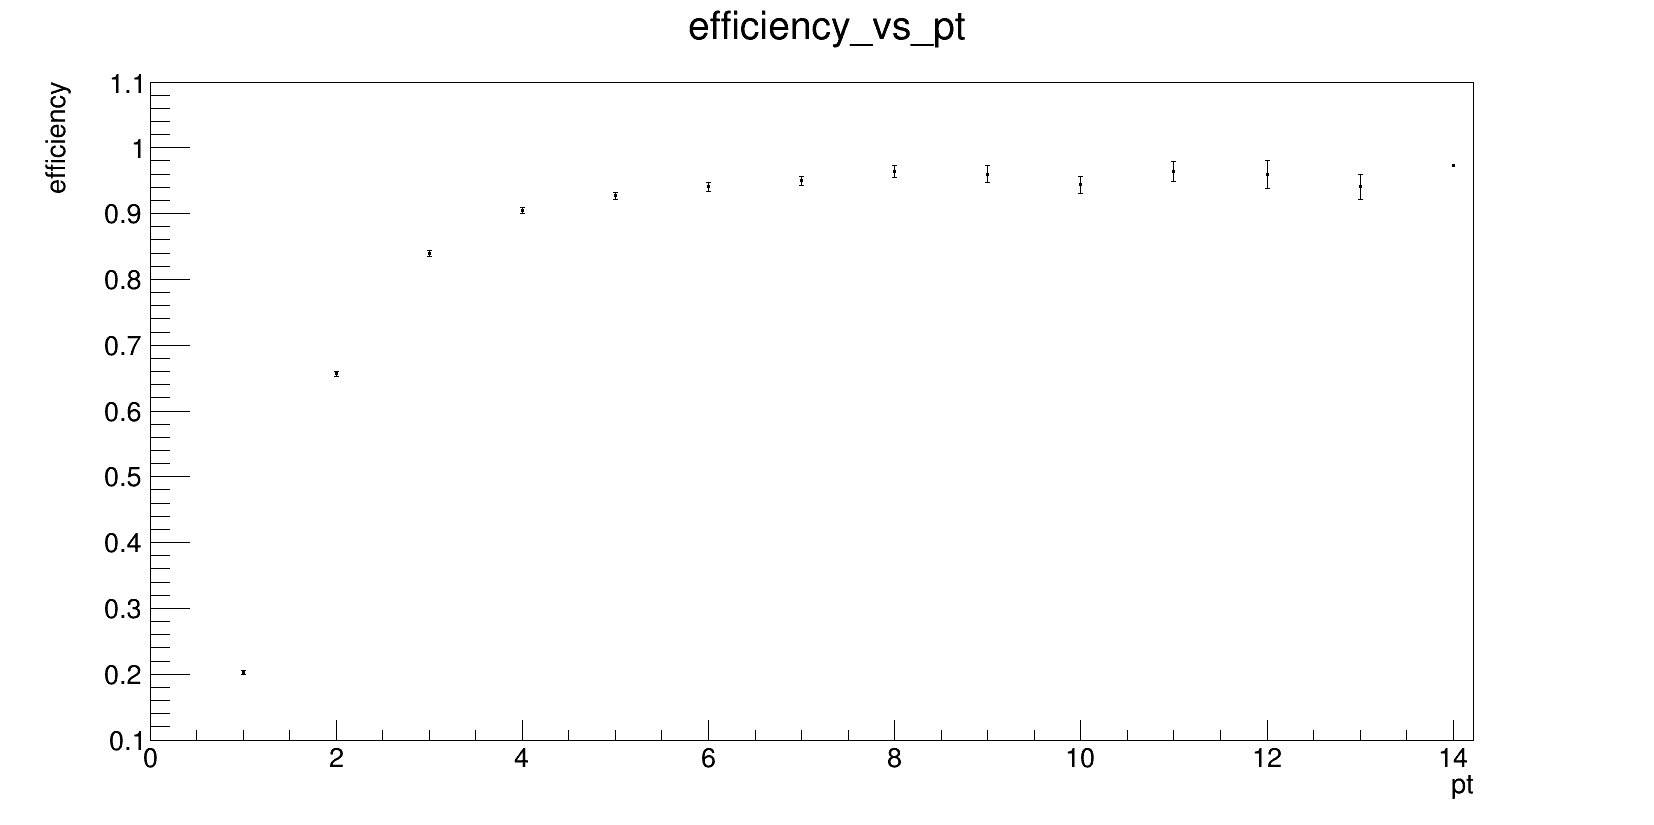
\includegraphics[scale=0.25]{rozdzial6/KsDD_pt.png} \\
\caption{Wydajność rekonstrukcji śladów typu downstream zrekonstruowanych dla cząstek z rozpadu $K_s \rightarrow \pi + \pi $  w funkcji pędu (góra), pędu poprzecznego (dół).}
\label{KsDD}
\end{figure}

Na rysunku \ref{effJPsi} przedstawiono zależności wydajności rekonstrukcji śladów długich pochodzących z rozpadu mezony $J\/Psi$.  Nie zauważono żadnych korelacji pomiędzy wartością parametrów pędu, pędu poprzecznego oraz pseudorapidity. Warto zwrócić uwagę na bardzo dobrą jakość rekonstrukcji śladów nawet dla małych wartości pędu, zarówno całkowitego jak i poprzecznego. W porównaniu do do rysunku \ref{effJPsi} sytuacja dla śladów stowarzyszonych z rozpadem mezonu $K_s \rightarrow \pi + \pi $ zarówno dla śladów długich jak i typu "downstream" jest inna. Wyraźnie widać zależność od pędu, dla małych jego wartości wydajność rekonstrukcji jest dość niska. Dopiero dla wartości pędu całkowitego większych od $40GeV/c^2$ rozkłady są praktycznie identyczne. 

Warto również przypatrzeć się niepewnością wyznaczenia wydajności rekonstrukcji. Łatwo zauważyć, że wzrasta ona wraz ze wzrostem wartości pędów, poprzecznego i całkowitego. Efekt ten jest łatwo wyjaśnić, gdyż dla takich wartości gwałtownie spada ilość rejestrowanych cząstek.  

\subsection{Rozkłady $\chi^2$}
\subsection{Zależności korelacyjne}
\section{Analiza oparta na danych}
\subsection{Rozkłady $\chi^2$ bazujące na danych}
\subsection{Ekstrakcja sygnału od szumu}
\subsection{Zależności korelacyjne}